\documentclass[../main]{subfiles}
\ifSubfilesClassLoaded{\setcounter{chapter}{5}}{}
\begin{document}

\chapter{Kriptografi Asimetris dan RSA}

\begin{subcpmk}
  \item Sub-CPMK 1.3: Mengenal kriptografi modern asimetris (RSA, Diffie--Hellman, ElGamal, pengantar ECC)
\end{subcpmk}

\noindent\textit{Rujukan:} Munir \cite{munir2019,munir_slides_itb}; HAC Bab~8 \cite{hac_online}; Katz \& Lindell \cite{katz2020}; Boneh \cite{boneh_cs255}.

% ============================================================
% MATERI POKOK
% ============================================================
\section{Konsep Kriptografi Asimetris dan Kunci Publik}

Dalam kriptografi asimetris, setiap pihak memiliki \textbf{pasangan kunci}: kunci publik (dapat dibagikan) dan kunci privat (rahasia). Enkripsi dengan kunci publik hanya dapat didekripsi dengan kunci privat yang sesuai. Sistem ini merevolusi cara komunikasi aman dengan menghilangkan kebutuhan untuk berbagi kunci rahasia melalui kanal yang aman.

Kriptografi asimetris pertama kali dipublikasikan oleh Whitfield Diffie dan Martin Hellman pada tahun 1976, yang membuka era baru dalam keamanan komunikasi digital. Menurut Wikipedia, konsep ini sangat revolusioner karena memungkinkan dua pihak yang belum pernah bertemu untuk berkomunikasi secara aman melalui jaringan publik. Ide dasar ini kemudian diimplementasikan secara praktis oleh Rivest, Shamir, dan Adleman dalam algoritma RSA yang menjadi fondasi kriptografi modern.

\textbf{Skema dasar}: Alice mempublikasikan kunci publik. Bob mengenkripsi pesan dengan kunci publik Alice. Hanya Alice (yang memiliki kunci privat) yang dapat mendekripsi. Sistem ini bekerja berdasarkan fungsi satu arah (one-way function) yang mudah dihitung dalam satu arah tetapi sangat sulit dibalikkan tanpa informasi rahasia.

\textbf{Manfaat}: Tidak perlu pertukaran kunci rahasia di kanal terbuka. Kunci publik dapat didistribusikan melalui direktori atau sertifikat. Menurut sumber keamanan, kemampuan untuk mendistribusikan kunci publik secara terbuka memungkinkan skala komunikasi aman yang sangat besar, seperti yang terlihat dalam internet modern dengan jutaan transaksi per hari.

\textbf{Keterbatasan}: Lebih lambat dibanding simetris. Umumnya digunakan untuk pertukaran kunci atau tanda tangan, bukan enkripsi data besar. Menurut Wikipedia, operasi matematika yang diperlukan untuk RSA (eksponensial modular) jauh lebih lambat dibandingkan operasi simetris seperti AES, sehingga penggunaan RSA untuk enkripsi data besar secara langsung tidak praktis.

\subsection{RSA untuk Enkripsi dan Tanda Tangan}

RSA dapat dipakai untuk \textbf{enkripsi} (gunakan kunci publik penerima) maupun \textbf{tanda tangan digital} (gunakan kunci privat pengirim). Keduanya memakai operasi modular yang sama, tetapi \textbf{tujuan dan padding} berbeda. Untuk enkripsi, skema yang direkomendasikan adalah RSAES-OAEP; untuk tanda tangan, skema yang direkomendasikan adalah RSASSA-PSS \cite{rfc8017}.

RSA dikembangkan oleh Ron Rivest, Adi Shamir, dan Leonard Adleman di MIT pada tahun 1977. Menurut Wikipedia, algoritma ini ditemukan setelah percobaan panjang selama satu tahun, dengan Rivest menghabiskan semalaman untuk memformalkan ide setelah tidak bisa tidur. Nama RSA berasal dari inisial nama belakang ketiga penemu dalam urutan yang sama seperti publikasi ilmiah mereka.

Secara praktik, RSA lebih sering digunakan untuk \textbf{key transport} (mengamankan kunci simetris) dan \textbf{signature}. Enkripsi data besar langsung dengan RSA tidak efisien dan dibatasi ukuran pesan, sehingga skema hybrid jauh lebih umum di sistem nyata. Menurut sumber keamanan, RSA dengan padding yang tepat (seperti OAEP) dapat membuktikan keamanannya secara matematis, tetapi implementasi yang salah dapat menyebabkan kerentanan yang serius.

\subsection{Hybrid Encryption dan KEM-DEM}

Karena RSA lambat, praktik umum adalah \textbf{hybrid encryption}: RSA hanya dipakai untuk mengamankan kunci simetris, sedangkan data utama dienkripsi dengan AES. Pola ini sering disebut \textbf{KEM-DEM} (Key Encapsulation Mechanism - Data Encapsulation Mechanism) \cite{nist800_56b_r2}:
\begin{enumerate}
  \item Buat kunci simetris acak $K_s$.
  \item Enkripsi pesan dengan AES (mis. GCM) menggunakan $K_s$ sehingga menghasilkan ciphertext $C$.
  \item Enkripsi $K_s$ dengan RSA-OAEP sehingga menghasilkan $C_K$.
  \item Kirimkan $(C_K, C)$ kepada penerima.
\end{enumerate}
Penerima mendekripsi $C_K$ untuk memperoleh $K_s$, lalu mendekripsi $C$ dengan AES.

Hybrid encryption menjadi standar industri karena menggabungkan keunggulan kedua jenis kriptografi. Menurut sumber keamanan, KEM-DEM menyediakan keamanan yang dapat dibuktikan (provable security) dengan efisiensi operasional yang tinggi. Pendekatan ini memungkinkan enkripsi data berukuran besar dengan kecepatan AES sambil mempertahankan keamanan kunci publik RSA untuk pertukaran kunci.

\begin{figure}[htbp]
  \centering
  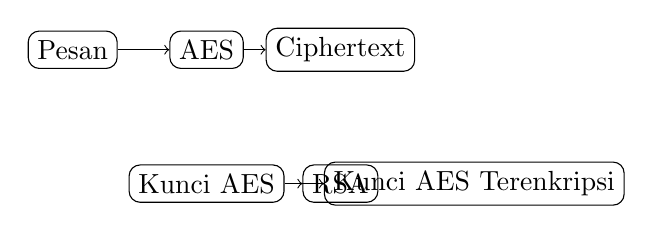
\begin{tikzpicture}[node distance=1.7cm]
    \node (msg) [draw, rounded corners] {Pesan};
    \node (aes) [draw, rounded corners, right of=msg] {AES};
    \node (ct) [draw, rounded corners, right of=aes] {Ciphertext};
    \node (key) [draw, rounded corners, below of=aes] {Kunci AES};
    \node (rsa) [draw, rounded corners, right of=key] {RSA};
    \node (ekey) [draw, rounded corners, right of=rsa] {Kunci AES Terenkripsi};
    \draw[->] (msg) -- (aes);
    \draw[->] (aes) -- (ct);
    \draw[->] (key) -- (rsa);
    \draw[->] (rsa) -- (ekey);
  \end{tikzpicture}
  \caption{Skema hybrid: RSA untuk kunci, AES untuk data.}
\end{figure}

\subsection{PKI dan Sertifikat}

Distribusi kunci publik membutuhkan \textbf{kepercayaan}. Dalam praktik, kunci publik dibungkus dalam sertifikat digital (PKI) agar identitas pemilik kunci dapat diverifikasi. Ini mencegah serangan \textit{man-in-the-middle} saat pertukaran kunci publik. Menurut Wikipedia, Public Key Infrastructure (PKI) menjadi fondasi untuk keamanan internet modern, memungkinkan verifikasi otomatis identitas digital.

PKI terdiri dari hierarki Certificate Authorities (CA) yang menerbitkan sertifikat digital setelah memverifikasi identitas pemohon. Menurut sumber keamanan, sertifikat mengandung kunci publik, informasi identitas, dan tanda tangan CA yang membuktikan keaslian. Sistem ini memungkinkan komunikasi aman antar pihak yang belum pernah bertemu, dengan kepercayaan yang didelegasikan melalui CA yang terpercaya.

\subsection{Validasi Kunci Publik dan Model Kepercayaan}

Saat menerima kunci publik (sertifikat), lakukan validasi dasar berikut:
\begin{itemize}
  \item Verifikasi rantai sertifikat sampai CA yang dipercaya.
  \item Cek masa berlaku, revocation (CRL/OCSP), dan penggunaan kunci (key usage).
  \item Pastikan identitas di sertifikat sesuai konteks (mis. domain atau identitas pengguna).
\end{itemize}
Tanpa validasi ini, enkripsi atau tanda tangan dapat mudah disusupi oleh kunci publik palsu.

Validasi sertifikat adalah langkah kritis dalam keamanan kriptografi asimetris. Menurut sumber keamanan, serangan man-in-the-middle berhasil ketika penyerang dapat menyisipkan kunci publik palsu yang dianggap sah oleh penerima. Proses validasi yang ketat, termasuk pemeriksaan Certificate Revocation Lists (CRL) dan Online Certificate Status Protocol (OCSP), sangat penting untuk mencegah penggunaan sertifikat yang telah dicabut.

\section{Contoh Lengkap RSA: Key Generation dan Enkripsi}

\subsection{Setup: Memilih Parameter}

Untuk memahami RSA secara konkret, kita akan menggunakan bilangan prima kecil. \textbf{Catatan}: Dalam praktik, gunakan prima 2048-bit atau lebih!

\textbf{Langkah 1: Pilih dua bilangan prima}
\begin{itemize}
  \item $p = 61$
  \item $q = 53$
\end{itemize}

\textbf{Verifikasi primalitas}: Kedua bilangan adalah prima.

\subsection{Key Generation Step-by-Step}

\textbf{Langkah 2: Hitung modulus $n$}
\begin{align*}
n &= p \times q \\
  &= 61 \times 53 \\
  &= 3233
\end{align*}

\textbf{Langkah 3: Hitung fungsi Euler $\phi(n)$}
\begin{align*}
\phi(n) &= (p-1)(q-1) \\
        &= 60 \times 52 \\
        &= 3120
\end{align*}

\textbf{Langkah 4: Pilih eksponen publik $e$}

Syarat: $1 < e < \phi(n)$ dan $\gcd(e, \phi(n)) = 1$

Pilih $e = 17$ (nilai umum: 3, 17, 65537)

Verifikasi: $\gcd(17, 3120) = 1$ $\checkmark$

\textbf{Langkah 5: Hitung eksponen privat $d$}

Cari $d$ sehingga $e \cdot d \equiv 1 \pmod{\phi(n)}$

Menggunakan Extended Euclidean Algorithm:
\begin{align*}
17 \cdot d &\equiv 1 \pmod{3120} \\
d &= e^{-1} \text{ mod } \phi(n) \\
  &= 2753
\end{align*}

\textbf{Verifikasi}:
\begin{align*}
17 \times 2753 &= 46801 \\
46801 \text{ mod } 3120 &= 1 \quad \checkmark
\end{align*}

\subsection{Kunci RSA yang Dihasilkan}

\begin{table}[htbp]
  \centering
  \begin{tabular}{ll}
    \toprule
    \textbf{Parameter} & \textbf{Nilai} \\
    \midrule
    Public Key $(e, n)$ & $(17, 3233)$ \\
    Private Key $(d, n)$ & $(2753, 3233)$ \\
    \midrule
    Prima $p$ & 61 (rahasia) \\
    Prima $q$ & 53 (rahasia) \\
    $\phi(n)$ & 3120 (rahasia) \\
    \bottomrule
  \end{tabular}
  \caption{Kunci RSA yang dihasilkan dari contoh.}
\end{table}

\subsection{Enkripsi Pesan}

\textbf{Plaintext}: $m = 123$ (harus $m < n$)

\textbf{Enkripsi}: $c = m^e \bmod n$

\begin{align*}
c &= 123^{17} \bmod 3233
\end{align*}

\textbf{Perhitungan menggunakan square-and-multiply}:

Eksponen $17 = 10001_2$ (binary)

\begin{table}[htbp]
  \centering
  \small
  \begin{tabular}{cccl}
    \toprule
    \textbf{Bit} & \textbf{Square} & \textbf{Multiply} & \textbf{Result} \\
    \midrule
    1 & - & $123^1$ & 123 \\
    0 & $123^2 = 15129 \bmod 3233$ & - & 855 \\
    0 & $855^2 = 731025 \bmod 3233$ & - & 2790 \\
    0 & $2790^2 = 7784100 \bmod 3233$ & - & 1084 \\
    1 & $1084^2 = 1175056 \bmod 3233$ & $\times 123$ & 2516 \\
    \bottomrule
  \end{tabular}
  \caption{Square-and-multiply untuk $123^{17} \bmod 3233$.}
\end{table}

\textbf{Ciphertext}: $c = 855$

\subsection{Dekripsi Pesan}

\textbf{Ciphertext}: $c = 855$

\textbf{Dekripsi}: $m = c^d \bmod n$

\begin{align*}
m &= 855^{2753} \bmod 3233
\end{align*}

Menggunakan square-and-multiply (eksponen besar, hanya hasil akhir):

\textbf{Plaintext yang didekripsi}: $m = 123$ $\checkmark$

\subsection{Verifikasi Kebenaran}

\begin{align*}
m &= (m^e)^d \bmod n \\
  &= m^{ed} \bmod n \\
  &= m^{ed \bmod \phi(n)} \bmod n \quad \text{(Euler's theorem)} \\
  &= m^1 \bmod n \\
  &= m
\end{align*}

Karena $ed = 17 \times 2753 = 46801 \equiv 1 \pmod{3120}$

\subsection{Contoh dengan Pesan Teks}

Untuk mengenkripsi teks, konversi ke angka terlebih dahulu:

\textbf{Plaintext}: "HI"
\begin{itemize}
  \item H = 72 (ASCII)
  \item I = 73 (ASCII)
\end{itemize}

\textbf{Enkripsi}:
\begin{align*}
c_1 &= 72^{17} \bmod 3233 = 1234 \\
c_2 &= 73^{17} \bmod 3233 = 2819
\end{align*}

\textbf{Ciphertext}: [1234, 2819]

\textbf{Dekripsi}:
\begin{align*}
m_1 &= 1234^{2753} \bmod 3233 = 72 \rightarrow \text{H} \\
m_2 &= 2819^{2753} \bmod 3233 = 73 \rightarrow \text{I}
\end{align*}

\textbf{Plaintext}: "HI" $\checkmark$

\subsection{Implementasi C untuk Contoh Ini}

\begin{lstlisting}[style=cstyle, caption={RSA dengan Parameter Kecil}]
#include <stdio.h>

// Modular exponentiation: (base^exp) % mod
long long mod_exp(long long base, long long exp, long long mod) {
    long long result = 1;
    base = base % mod;
    
    while (exp > 0) {
        if (exp % 2 == 1) {
            result = (result * base) % mod;
        }
        exp = exp >> 1;
        base = (base * base) % mod;
    }
    
    return result;
}

int main() {
    long long n = 3233;
    long long e = 17;
    long long d = 2753;
    
    // Plaintext
    long long m = 123;
    printf("Plaintext: %lld\n", m);
    
    // Encryption
    long long c = mod_exp(m, e, n);
    printf("Ciphertext: %lld\n", c);
    
    // Decryption
    long long decrypted = mod_exp(c, d, n);
    printf("Decrypted: %lld\n", decrypted);
    
    return 0;
}
\end{lstlisting}

\textbf{Output}:
\begin{verbatim}
Plaintext: 123
Ciphertext: 855
Decrypted: 123
\end{verbatim}

\begin{catatan}
Contoh ini menggunakan bilangan prima kecil untuk tujuan edukatif. Dalam praktik:
\begin{itemize}
  \item Gunakan prima 2048-bit atau lebih (RSA-2048, RSA-4096)
  \item Gunakan padding scheme seperti OAEP untuk keamanan
  \item Jangan enkripsi data panjang langsung dengan RSA (gunakan hybrid encryption)
  \item Gunakan library kriptografi yang sudah diaudit (OpenSSL, libsodium)
\end{itemize}
\end{catatan}

\subsection{Mengapa RSA Aman?}

Keamanan RSA bergantung pada kesulitan \textbf{faktorisasi bilangan besar}:

\begin{itemize}
  \item Publik tahu: $n = 3233$, $e = 17$
  \item Untuk menemukan $d$, penyerang harus:
    \begin{enumerate}
      \item Faktorkan $n = 3233$ menjadi $p \times q$
      \item Hitung $\phi(n) = (p-1)(q-1)$
      \item Hitung $d = e^{-1} \bmod \phi(n)$
    \end{enumerate}
  \item Untuk $n$ kecil (3233), ini mudah: $3233 = 61 \times 53$
  \item Untuk $n$ besar (2048-bit), ini \textbf{sangat sulit} dengan teknologi saat ini
\end{itemize}

\textbf{Contoh kompleksitas}:
\begin{itemize}
  \item RSA-768 (232 digit): difaktorkan tahun 2009 setelah 2 tahun komputasi
  \item RSA-2048 (617 digit): diperkirakan butuh jutaan tahun dengan teknologi saat ini
\end{itemize}

\section{Algoritma RSA}

\begin{subcpmk}
  \item Mahasiswa mampu menganalisis derivasi matematis algoritma RSA, membuktikan koreksi dekripsinya melalui Teorema Euler, melakukan proses pembuatan kunci, enkripsi, dan dekripsi secara manual, serta mengevaluasi kompleksitas komputasinya.
\end{subcpmk}

\noindent\textit{Rujukan:} Munir \cite{munir2019,munir_slides_itb}; HAC Bab~8 \cite{hac_online}; Katz \& Lindell \cite{katz2020}; Boneh \cite{boneh_cs255}.

\subsection{Landasan Matematis: Fungsi Totient dan Teorema Euler}

RSA (Rivest-Shamir-Adleman) adalah algoritma kunci publik pertama yang mengimplementasikan konsep \textit{trapdoor one-way function} menggunakan operasi aritmetika modular. Keamanan RSA bersandar pada \textbf{Integer Factorization Problem} (IFP): fakta bahwa mengalikan dua bilangan prima besar sangat mudah, tetapi memfaktorkan hasil kalinya kembali menjadi dua prima asalnya secara komputasi mustahil untuk bilangan yang sangat besar.

Dua konsep matematika kunci yang mendasari RSA adalah:

\begin{enumerate}
    \item \textbf{Fungsi Totient Euler $\varphi(n)$}: Fungsi ini menghitung jumlah bilangan bulat positif kurang dari $n$ yang koprima dengan $n$. Jika $n = p \cdot q$ dan $p, q$ adalah bilangan prima, maka:
    \begin{equation}
      \varphi(n) = (p-1)(q-1)
    \end{equation}

    \item \textbf{Teorema Euler}: Jika $\gcd(a, n) = 1$, maka:
    \begin{equation}
      a^{\varphi(n)} \equiv 1 \pmod{n}
    \end{equation}
\end{enumerate}

\subsection{Prosedur Algoritma RSA}

Proses RSA terbagi menjadi tiga tahap: pembangkitan kunci, enkripsi, dan dekripsi.

\subsubsection{Pembangkitan Kunci (Key Generation)}
\begin{enumerate}
    \item Pilih dua bilangan prima besar $p$ dan $q$ secara acak dan independen.
    \item Hitung $n = p \cdot q$. Nilai $n$ disebut sebagai \textit{modulus} dan panjangnya dalam bit menentukan kekuatan kunci.
    \item Hitung $\varphi(n) = (p-1)(q-1)$.
    \item Pilih bilangan bulat $e$ sedemikian sehingga $1 < e < \varphi(n)$ dan $\gcd(e, \varphi(n)) = 1$. Nilai $e$ adalah \textit{public exponent}. Nilai standar yang umum digunakan adalah $e = 65537$ ($2^{16}+1$) karena efisien untuk komputasi.
    \item Hitung $d$ sebagai invers multiplikatif modular dari $e$ modulo $\varphi(n)$, sehingga:
    \begin{equation}
      e \cdot d \equiv 1 \pmod{\varphi(n)}
    \end{equation}
    Nilai $d$ dihitung menggunakan \textbf{Algoritma Euclidean Diperluas} (EEA).
\end{enumerate}
\textbf{Kunci Publik}: $(e, n)$ \\
\textbf{Kunci Privat}: $(d, n)$ atau cukup $(d)$

\subsubsection{Enkripsi}
Untuk pesan $M$ yang dinyatakan sebagai bilangan bulat $0 \le M < n$, cipherteks $C$ dihitung dengan:
\begin{equation}
  C = M^e \pmod{n}
\end{equation}

\subsubsection{Dekripsi}
Penerima menggunakan kunci privat $d$ untuk memulihkan pesan $M$ dari cipherteks $C$:
\begin{equation}
  M = C^d \pmod{n}
\end{equation}

\subsection{Pembuktian Koreksi RSA}

Untuk membuktikan bahwa dekripsi selalu mengembalikan pesan asli, kita harus menunjukkan bahwa $C^d \equiv M \pmod{n}$.

\begin{proof}
Berdasarkan definisi enkripsi:
\[ C^d \equiv (M^e)^d \equiv M^{ed} \pmod{n} \]
Karena $e \cdot d \equiv 1 \pmod{\varphi(n)}$, maka terdapat bilangan bulat $k$ sedemikian sehingga $ed = k\varphi(n) + 1$.
\[ M^{ed} = M^{k\varphi(n) + 1} = (M^{\varphi(n)})^k \cdot M^1 \]
Menurut Teorema Euler, $M^{\varphi(n)} \equiv 1 \pmod{n}$ (asumsi $M$ koprima dengan $n$):
\[ M^{ed} \equiv (1)^k \cdot M \equiv M \pmod{n} \]
Jika $M$ tidak koprima dengan $n$ (kasus yang sangat jarang untuk $p, q$ besar), pembuktian tetap berlaku menggunakan Teorema Sisa Tionghoa (CRT). Jadi, proses dekripsi selalu benar.
\end{proof}

\subsection{Contoh Perhitungan Manual (Small-Scale RSA)}

Misalkan kita ingin mengimplementasikan RSA dengan bilangan prima kecil:
\begin{enumerate}
    \item \textbf{Kunci}: Pilih $p = 11, q = 13 \rightarrow n = 143$.
    \item \textbf{Totient}: $\varphi(143) = (10)(12) = 120$.
    \item \textbf{Eksponen Publik}: Pilih $e = 7$ (cek $\gcd(7, 120) = 1 \checkmark$).
    \item \textbf{Eksponen Privat}: Cari $d$ sehingga $7d \equiv 1 \pmod{120}$.
    Menggunakan EEA: $120 = 17 \cdot 7 + 1 \rightarrow 1 = 120(1) - 17(7)$.
    Maka $d \equiv -17 \equiv 103 \pmod{120}$.
\end{enumerate}
Kunci Publik: $(7, 143)$, Kunci Privat: $(103, 143)$.

\textbf{Proses Enkripsi}: Pesan $M = 9$.
\[ C = 9^7 \pmod{143} = 4,782,969 \pmod{143} = 48 \]

\textbf{Proses Dekripsi}: Cipherteks $C = 48$.
\[ M = 48^{103} \pmod{143} = 9 \]

\subsection{Kompleksitas Komputasi dan Efisiensi}

Operasi utama dalam RSA adalah \textit{modular exponentiation} ($M^e \bmod n$). Jika dilakukan secara naif, kompleksitasnya adalah $\mathcal{O}(e)$, yang tidak praktis untuk $e$ besar. Oleh karena itu, digunakan algoritma \textbf{Square-and-Multiply} (atau \textit{Binary Exponentiation}) yang mereduksi kompleksitas menjadi $\mathcal{O}(\log e)$.

\begin{figure}[htbp]
  \centering
  \includegraphics[width=0.7\textwidth]{bab-06/rsa-square-multiply-diagram}
  \caption{Alur kerja algoritma Square-and-Multiply untuk eksponensiasi modular efisien.}
  \label{fig:rsa-square-multiply}
\end{figure}

\subsection{Keamanan dan Padding OAEP}

\textit{Textbook RSA} (RSA tanpa padding) memiliki kelemahan fatal:
\begin{enumerate}
    \item \textbf{Deterministik}: Pesan yang sama selalu menghasilkan cipherteks yang sama.
    \item \textbf{Kerentanan Matematis}: Jika $M$ kecil dan $e=3$, maka $M^3$ mungkin kurang dari $n$, sehingga $M$ dapat ditemukan dengan akar pangkat tiga biasa.
\end{enumerate}
Untuk mengatasinya, standar industri menggunakan \textbf{Optimal Asymmetric Encryption Padding (OAEP)}. OAEP menambahkan struktur acak (menggunakan fungsi hash) ke dalam pesan sebelum dienkripsi, sehingga mengubah RSA menjadi skema enkripsi probabilistik: pesan yang sama akan menghasilkan cipherteks berbeda setiap kali dienkripsi.

\begin{aktivitas}
  \item \textbf{Eksperimen RSA}: Implementasikan algoritma Square-and-Multiply dalam bahasa Python. Bandingkan waktu eksekusi antara metode perkalian berulang naif dengan metode Square-and-Multiply untuk eksponen $e > 10^6$.
\end{aktivitas}

\begin{latihan}
  \item Diketahui $p=17, q=19, e=5$. Hitunglah $n, \varphi(n), d$, kunci publik, dan kunci privat!
  \item Lakukan enkripsi dan dekripsi untuk pesan $M=10$ menggunakan parameter pada soal nomor 1!
  \item Mengapa pemilihan $e = 65537$ sangat populer dalam implementasi RSA? Jelaskan dari sisi efisiensi biner!
  \item Jika seorang penyerang berhasil menemukan $\varphi(n)$, apakah ia dapat memecahkan RSA? Jelaskan langkah-langkah yang akan dilakukan penyerang tersebut!
\end{latihan}

\section{Diffie-Hellman, ElGamal, dan Pengantar ECC}

\subsection{Diffie-Hellman Key Exchange}

Diffie-Hellman memungkinkan dua pihak untuk \textbf{menyetujui kunci rahasia bersama} melalui kanal tidak aman \cite{stallings2017}. Parameter publik: bilangan prima $p$ dan generator $g$ dari $\mathbb{Z}_p^*$.

\begin{enumerate}
  \item Alice memilih $a$ acak, menghitung $A = g^a \bmod p$, mengirim $A$ ke Bob.
  \item Bob memilih $b$ acak, menghitung $B = g^b \bmod p$, mengirim $B$ ke Alice.
  \item Alice menghitung $K = B^a \bmod p = g^{ab} \bmod p$.
  \item Bob menghitung $K = A^b \bmod p = g^{ab} \bmod p$.
\end{enumerate}

Keduanya memperoleh $K = g^{ab} \bmod p$. Penyerang yang melihat $A$, $B$, $g$, $p$ harus menyelesaikan \textbf{masalah Diffie-Hellman}: hitung $g^{ab}$ dari $g^a$ dan $g^b$, yang setara dengan logaritma diskrit \cite{menezes1996}.

\begin{figure}[htbp]
  \centering
  \begin{tikzpicture}[node distance=1.2cm]
    \node[draw] (alice) {Alice};
    \node[draw, right=3cm of alice] (bob) {Bob};
    \node[below=0.6cm of alice, font=\small] {$a$, $A=g^a$};
    \node[below=0.6cm of bob, font=\small] {$b$, $B=g^b$};
    \draw[->] (alice) -- node[above] {$A$} (bob);
    \draw[->] (bob) -- node[below] {$B$} (alice);
    \node[below=1.8cm of alice, font=\small] {$K=A^b=g^{ab}$};
    \node[below=1.8cm of bob, font=\small] {$K=B^a=g^{ab}$};
  \end{tikzpicture}
  \caption{Diffie-Hellman: pertukaran $A$, $B$; kunci bersama $K=g^{ab}$.}
\end{figure}

\begin{catatan}
Diffie-Hellman sendiri tidak memberikan otentikasi; rentan man-in-the-middle. Digunakan dalam protokol seperti TLS dengan otentikasi sertifikat.
\end{catatan}

\subsection{ElGamal}

ElGamal adalah skema enkripsi berbasis logaritma diskrit \cite{stallings2017}. Parameter: prima $p$, generator $g$.

\textbf{Pembangkitan kunci}: Pilih $x$ acak (privat), hitung $y = g^x \bmod p$ (publik). Kunci publik $(p, g, y)$; kunci privat $x$.

\textbf{Enkripsi} pesan $m$: Pilih $k$ acak, hitung $c_1 = g^k \bmod p$ dan $c_2 = m \cdot y^k \bmod p$. Ciphertext $(c_1, c_2)$.

\textbf{Dekripsi}: $m = c_2 \cdot (c_1^x)^{-1} \bmod p = c_2 \cdot (g^{xk})^{-1} \bmod p = m \cdot y^k \cdot (g^{xk})^{-1} = m$.

ElGamal bersifat probabilistik (bergantung pada $k$ acak). Keamanan bergantung pada kesulitan logaritma diskrit \cite{menezes1996}.

\subsection{Pengantar Elliptic Curve Cryptography (ECC)}

ECC menggunakan grup titik pada kurva eliptik atas field hingga \cite{stallings2017}. Masalah yang mendasari: \textbf{Elliptic Curve Discrete Logarithm Problem (ECDLP)}—diberikan titik $P$ dan $Q = kP$, cari $k$.

Keunggulan: keamanan setara dengan ukuran kunci lebih pendek. Kunci ECC 256-bit setara dengan RSA 3072-bit \cite{nist800_56b_r2}. Digunakan dalam TLS, Bitcoin, dll.

Algoritma ECC: ECDH (pertukaran kunci), ECDSA (tanda tangan), ECIES (enkripsi). Implementasi memerlukan aritmetika kurva eliptik; gunakan library (OpenSSL, libsodium) \cite{menezes1996}.


\section{Implementasi RSA dalam C}

Implementasi RSA yang aman memerlukan perhatian pada side-channel dan operasi constant-time \cite{ferguson2010}. Untuk pembelajaran gunakan bilangan kecil; untuk produksi gunakan library (OpenSSL, GMP).

\subsection{Implementasi Edukatif dengan Bilangan Kecil}

Implementasi sederhana berguna untuk memahami konsep dasar RSA:
\begin{lstlisting}[style=cstyle, caption={RSA Sederhana dengan Bilangan Kecil (C)}]
#include <stdio.h>

long long mod_pow(long long base, long long exp, long long mod) {
    long long result = 1;
    base = base % mod;
    while (exp > 0) {
        if (exp % 2 == 1) result = (result * base) % mod;
        exp /= 2;
        base = (base * base) % mod;
    }
    return result;
}

int main() {
    long long p = 61, q = 53;
    long long n = p * q;
    long long phi = (p-1) * (q-1);
    long long e = 17;
    long long d = 2753;  /* e^(-1) mod phi, precomputed */
    
    long long m = 65;  /* plaintext */
    long long c = mod_pow(m, e, n);
    long long m2 = mod_pow(c, d, n);
    
    printf("Plaintext: %lld\n", m);
    printf("Ciphertext: %lld\n", c);
    printf("Decrypted: %lld\n", m2);
    return 0;
}
\end{lstlisting}

Kode di atas hanya untuk pembelajaran; tidak memiliki padding aman atau constant-time operations.

\subsection{Implementasi Produksi dengan OpenSSL}

Untuk RSA nyata, gunakan API OpenSSL berbasis \code{EVP\_PKEY} dan padding OAEP/PSS \cite{rfc8017}.

\begin{lstlisting}[style=cstyle, caption={Cuplikan EVP untuk RSA-OAEP (ringkas)}]
EVP_PKEY_CTX *ctx = EVP_PKEY_CTX_new(pkey, NULL);
EVP_PKEY_encrypt_init(ctx);
EVP_PKEY_CTX_set_rsa_padding(ctx, RSA_PKCS1_OAEP_PADDING);
EVP_PKEY_CTX_set_rsa_oaep_md(ctx, EVP_sha256());
EVP_PKEY_encrypt(ctx, out, &outlen, in, inlen);
\end{lstlisting}

\begin{lstlisting}[style=cstyle, caption={Cuplikan EVP untuk RSA-PSS (ringkas)}]
EVP_PKEY_CTX *ctx = EVP_PKEY_CTX_new(pkey, NULL);
EVP_PKEY_sign_init(ctx);
EVP_PKEY_CTX_set_rsa_padding(ctx, RSA_PKCS1_PSS_PADDING);
EVP_PKEY_CTX_set_signature_md(ctx, EVP_sha256());
EVP_PKEY_sign(ctx, sig, &siglen, msg, msglen);
\end{lstlisting}


\subsection{Keamanan Implementasi dan Side-Channel Attacks}

Implementasi RSA yang aman harus memperhatikan berbagai aspek keamanan:
\begin{itemize}
  \item \textbf{Random Number Generation}: Gunakan RNG kriptografis yang kuat untuk kunci dan salt.
  \item \textbf{Constant-Time Operations}: Implementasi operasi modular yang waktu eksekusinya konstan.
  \item \textbf{Blinding}: Gunakan cryptographic blinding untuk melindungi dari timing attacks.
  \item \textbf{Memory Security}: Hapus sensitif data dari memory setelah digunakan.
  \item \textbf{Input Validation}: Validasi semua input sebelum diproses.
\end{itemize}

Timing attacks (Kocher, 1995) dapat mendeduksi kunci dari waktu dekripsi. Gunakan constant-time dan blinding \cite{ferguson2010}.

\subsection{Cryptographic Blinding}

Cryptographic blinding melindungi dari timing attacks.

Implementasi blinding dalam RSA:
\begin{enumerate}
  \item Pilih nilai acak $r$ untuk setiap operasi dekripsi
  \item Hitung $c' = c \cdot r^e \bmod n$
  \item Lakukan dekripsi: $m' = (c')^d \bmod n$
  \item Hilangkan blinding: $m = m' \cdot r^{-1} \bmod n$
\end{enumerate}


\subsection{Optimasi Performa dengan Chinese Remainder Theorem}

Optimasi CRT memberikan percepatan hingga 4x untuk dekripsi.

\begin{lstlisting}[style=cstyle, caption={Optimasi CRT untuk RSA Dekripsi}]
// Precompute CRT parameters
long long dP = d % (p-1);
long long dQ = d % (q-1);
long long qInv = mod_inverse(q, p);

// CRT-based decryption
long long m1 = mod_pow(c, dP, p);
long long m2 = mod_pow(c, dQ, q);
long long h = ((qInv * (m1 - m2)) % p) * q;

long long m = (m2 + h) % n;
\end{lstlisting}


\subsection{Validasi dan Testing}

Implementasi RSA harus divalidasi secara menyeluruh sebelum digunakan dalam produksi:
\begin{itemize}
  \item \textbf{Known Answer Tests}: Uji dengan vektor test yang telah dipublikasikan.
  \item \textbf{Randomized Tests}: Uji dengan input acak untuk mendeteksi bug.
  \item \textbf{Side-Channel Tests}: Uji resistensi terhadap timing dan cache attacks.
  \item \textbf{Performance Tests}: Uji throughput dan latensi untuk berbagai ukuran kunci.
\end{itemize}


\section{Elliptic Curve Cryptography (ECC)}

\subsection{Pengantar Elliptic Curve}

Elliptic Curve Cryptography (ECC) adalah alternatif modern untuk RSA yang menawarkan keamanan setara dengan ukuran kunci yang jauh lebih kecil \cite{hankerson2004}. ECC didasarkan pada matematika kurva eliptik atas field hingga, memberikan keamanan yang lebih efisien untuk perangkat dengan sumber daya terbatas seperti smartphone dan IoT devices.

\textbf{Keunggulan ECC vs RSA}:
\begin{itemize}
  \item \textbf{Ukuran kunci}: ECC 256-bit $\approx$ RSA 3072-bit dalam keamanan
  \item \textbf{Efisiensi komputasi}: Operasi ECC lebih cepat untuk ukuran kunci yang sama
  \item \textbf{Ukuran signature}: ECC signature lebih kecil
  \item \textbf{Implementasi}: Cocok untuk perangkat dengan sumber daya terbatas
\end{itemize}

\subsection{Kurva Eliptik atas Field Hingga}

Kurva eliptik atas field hingga $\mathbb{F}_p$ didefinisikan sebagai:
\[
E: y^2 = x^3 + ax + b \pmod{p}
\]
dimana $4a^3 + 27b^2 \neq 0 \pmod{p}$ (tidak ada singularitas).

\begin{contoh}
Kurva secp256r1 (NIST P-256):
\begin{itemize}
  \item Prime field: $p = 2^{256} - 2^{224} + 2^{192} + 2^{96} - 1$
  \item Kurva: $y^2 = x^3 - 3x + b \pmod{p}$
  \item Koefisien $b$: \path{0x5AC635D8AA3A93E7B3EBBD55769886BC651D06B0CC53B0F63BCE3C3E27D2604B}
\end{itemize}
\end{contoh}

\subsection{Struktur Aljabar Kurva Eliptik}

Himpunan titik pada kurva eliptik membentuk grup abelian dengan operasi penjumlahan titik \cite{silverman2009}:

\textbf{Elemen Identitas}: Titik di tak hingga $\mathcal{O}$

\textbf{Penjumlahan Titik}: Diberikan dua titik $P$ dan $Q$, penjumlahan $P + Q$ didefinisikan sebagai:
\begin{enumerate}
  \item Jika $P = \mathcal{O}$, maka $P + Q = Q$
  \item Jika $Q = \mathcal{O}$, maka $P + Q = P$
  \item Jika $x_P = x_Q$ dan $y_P = -y_Q$, maka $P + Q = \mathcal{O}$ (invers)
  \item Jika tidak, maka garis melalui $P$ dan $Q$ memotong kurva di titik ketiga $R$, dan $P + Q$ adalah refleksi $R$ terhadap sumbu x
\end{enumerate}

\textbf{Perkalian Titik}: Perkalian skalar $kP$ adalah penjumlahan titik $P$ dengan dirinya sendiri sebanyak $k$ kali:
\[
kP = \underbrace{P + P + \cdots + P}_{k \text{ kali}}
\]

\begin{figure}[htbp]
  \centering
  \begin{tikzpicture}[scale=0.8]
    % Draw axes
    \draw[->] (-3,0) -- (4,0) node[right] {$x$};
    \draw[->] (0,-2) -- (3,2) node[above] {$y$};
    
    % Draw elliptic curve y^2 = x^3 - 3x + 1 (non-negative for x in ~[-1.88,0.35] and [1.54,infty))
    \draw[thick, blue] plot[smooth, domain=-1.86:0.34] (\x, {sqrt(\x*\x*\x - 3*\x + 1)});
    \draw[thick, blue] plot[smooth, domain=-1.86:0.34] (\x, {-sqrt(\x*\x*\x - 3*\x + 1)});
    \draw[thick, blue] plot[smooth, domain=1.54:3.5] (\x, {sqrt(\x*\x*\x - 3*\x + 1)});
    \draw[thick, blue] plot[smooth, domain=1.54:3.5] (\x, {-sqrt(\x*\x*\x - 3*\x + 1)});
    
    % Draw points
    \node[circle, fill=red, inner sep=2pt] (P) at (1,1) {};
    \node[below right] at (P) {$P$};
    
    \node[circle, fill=red, inner sep=2pt] (Q) at (-1,1) {};
    \node[below left] at (Q) {$Q$};
    
    \node[circle, fill=green, inner sep=2pt] (R) at (2,-2) {};
    \node[below] at (R) {$R$};
    
    \node[circle, fill=green, inner sep=2pt] (PplusQ) at (2,2) {};
    \node[above] at (PplusQ) {$P+Q$};
    
    % Draw lines
    \draw[dashed, red] (P) -- (Q);
    \draw[dashed, green] (PplusQ) -- (R);
  \end{tikzpicture}
  \caption{Penjumlahan titik pada kurva eliptik: $P + Q = R'$}
\end{figure}

\subsection{Implementasi Operasi Kurva Eliptik}

\subsubsection{Representasi Titik}

Titik pada kurva eliptik direpresentasikan sebagai struktur:
\begin{lstlisting}[style=cstyle, caption={Representasi Titik ECC}]
typedef struct {
    int x;
    int y;
    int is_infinity;  // flag untuk titik di tak hingga
} ECPoint;
\end{lstlisting}

\subsubsection{Penjumlahan Titik dalam C}

\begin{lstlisting}[style=cstyle, caption={Penjumlahan Titik Kurva Eliptik}]
ECPoint point_add(ECPoint P, ECPoint Q, int p, int a, int b) {
    ECPoint R;
    
    if (P.is_infinity) return Q;
    if (Q.is_infinity) return P;
    
    // Check for invers
    if (P.x == Q.x && P.y == -Q.y % p) {
        R.is_infinity = 1;
        return R;
    }
    
    // Calculate slope
    int lambda;
    if (P.x == Q.x) {
        // Point doubling: 2P
        lambda = (3 * P.x * P.x + a) * mod_inverse(2 * P.y, p) % p;
    } else {
        // Point addition: P + Q
        lambda = (Q.y - P.y) * mod_inverse(Q.x - P.x, p) % p;
    }
    
    // Calculate result
    R.x = (lambda * lambda - P.x - Q.x) % p;
    R.y = (lambda * (P.x - R.x) - P.y) % p;
    R.is_infinity = 0;
    
    return R;
}
\end{lstlisting}

\subsubsection{Perkalian Skalar dengan Double-and-Add}

\begin{lstlisting}[style=cstyle, caption={Perkalian Skalar dengan Double-and-Add}]
ECPoint scalar_multiply(ECPoint P, int k, int p, int a, int b) {
    ECPoint result;
    result.is_infinity = 1;  // Initialize to infinity
    
    ECPoint current = P;
    
    while (k > 0) {
        if (k & 1) {
            result = point_add(result, current, p, a, b);
        }
        current = point_add(current, current, p, a, b);  // Double
        k >>= 1;
    }
    
    return result;
}
\end{lstlisting}

\subsection{Domain Parameters ECC}

Setiap kurva eliptik memiliki domain parameters yang didefinisikan secara unik:

\begin{table}[htbp]
  \centering
  \small
  \begin{tabular}{ll}
    \toprule
    Parameter & Deskripsi \\
    \midrule
    $p$ & Prime modulus field \\
    $a, b$ & Koefisien kurva $y^2 = x^3 + ax + b$ \\
    $G$ & Generator point (base point) \\
    $n$ & Order generator (jumlah titik dalam grup) \\
    $h$ & Cofactor $h = \#E(\mathbb{F}_p)/n$ \\
    \bottomrule
  \end{tabular}
  \caption{Domain parameters kurva eliptik.}
\end{table}

\begin{contoh}
Domain parameters secp256r1 (NIST P-256):
\begin{itemize}
  \item $p$ = \path{0xFFFFFFFF00000001000000000000000000000000FFFFFFFFFFFFFFFFFFFFFFFF}
  \item $a$ = \path{0xFFFFFFFF00000001000000000000000000000000FFFFFFFFFFFFFFFFFFFFFFFC}
  \item $b$ = \path{0x5AC635D8AA3A93E7B3EBBD55769886BC651D06B0CC53B0F63BCE3C3E27D2604B}
  \item $G_x$ = \path{0x6B17D1F2E12C4247F8BCE6E563A440F277037D812DEB33A0F4A13945D898C296}
  \item $G_y$ = \path{0x4FE342E2FE1A7F9B8EE7EB4A7C0F9E162BCE33576B315ECECBB6406837BF51F5}
  \item $n$ = \path{0xFFFFFFFF00000000FFFFFFFFFFFFFFFFBCE6FAADA7179E84F3B9CAC2FC632551}
  \item $h$ = 1
\end{itemize}
\end{contoh}

\subsection{ECC untuk Kriptografi Kunci Publik}

\subsubsection{ECDSA (Elliptic Curve Digital Signature Algorithm)}

ECDSA adalah adaptasi DSA untuk kurva eliptik \cite{johnson2001}:

\textbf{Key Generation}:
\begin{enumerate}
  \item Pilih bilangan acak $d$ dengan $1 < d < n$
  \item Hitung kunci publik $Q = dG$
  \item Private key: $d$, Public key: $Q$
\end{enumerate}

\textbf{Signature Generation}:
\begin{enumerate}
  \item Pilih bilangan acak $k$ dengan $1 < k < n$
  \item Hitung $R = kG = (x_R, y_R)$
  \item Hitung $r = x_R \bmod n$
  \item Hitung $s = k^{-1}(H(m) + dr) \bmod n$
  \item Signature: $(r, s)$
\end{enumerate}

\textbf{Signature Verification}:
\begin{enumerate}
  \item Hitung $w = s^{-1} \bmod n$
  \item Hitung $u_1 = H(m)w \bmod n$
  \item Hitung $u_2 = rw \bmod n$
  \item Hitung $X = u_1G + u_2Q = (x_X, y_X)$
  \item Hitung $v = x_X \bmod n$
  \item Valid jika $v = r$
\end{enumerate}

\subsubsection{ECDH (Elliptic Curve Diffie-Hellman)}

ECDH adalah protokol pertukaran kunci berdasarkan kurva eliptik \cite{menezes1996}:

\textbf{Key Exchange}:
\begin{enumerate}
  \item Alice memilih $a$ acak, hitung $A = aG$
  \item Bob memilih $b$ acak, hitung $B = bG$
  \item Alice mengirim $A$ ke Bob, Bob mengirim $B$ ke Alice
  \item Alice hitung $K = aB$, Bob hitung $K = bA$
  \item Keduanya mendapatkan kunci bersama yang sama
\end{enumerate}

\begin{lstlisting}[style=cstyle, caption={ECDH Key Exchange}]
// Alice's side
int a = random_int(1, n-1);
ECPoint A = scalar_multiply(G, a, p, curve_a, curve_b);

// Bob's side  
int b = random_int(1, n-1);
ECPoint B = scalar_multiply(G, b, p, curve_a, curve_b);

// Shared secret computation
ECPoint shared_alice = scalar_multiply(B, a, p, curve_a, curve_b);
ECPoint shared_bob = scalar_multiply(A, b, p, curve_a, curve_b);

// Both should get the same point
assert(shared_alice.x == shared_bob.x && shared_alice.y == shared_bob.y);
\end{lstlisting}

\subsection{Keamanan ECC}

Keamanan ECC bergantung pada \textbf{Elliptic Curve Discrete Logarithm Problem} (ECDLP):
\begin{itemize}
  \item Diberikan $P$ dan $Q = kP$, sangat sulit menghitung $k$
  \item Tidak ada algoritma sub-eksponensial yang diketahui untuk ECDLP
  \item Pollard's rho algorithm adalah yang tercepat dengan kompleksitas $O(\sqrt{n})$
\end{itemize}

\begin{table}[htbp]
  \centering
  \small
  \begin{tabular}{lcc}
    \toprule
    Algoritma & Ukuran Kunci & Keamanan Setara \\
    \midrule
    RSA-1024 & 1024 bit & ECC-160 \\
    RSA-2048 & 2048 bit & ECC-224 \\
    RSA-3072 & 3072 bit & ECC-256 \\
    RSA-7680 & 7680 bit & ECC-384 \\
    RSA-15360 & 15360 bit & ECC-512 \\
    \bottomrule
  \end{tabular}
  \caption{Perbandingan keamanan RSA vs ECC.}
\end{table}

\subsection{Implementasi Praktis}

\textbf{Library yang Direkomendasikan}:
\begin{itemize}
  \item OpenSSL: Implementasi lengkap ECC (ECDSA, ECDH, EdDSA)
  \item libsodium: API modern dan aman untuk kriptografi
  \item Bouncy Castle: Library Java untuk kriptografi
  \item wolfSSL: Library C yang ringan untuk embedded systems
\end{itemize}

\textbf{Pertimbangan Implementasi}:
\begin{itemize}
  \item Gunakan kurva yang telah divalidasi (secp256r1, secp384r1, curve25519)
  \item Gunakan RNG yang aman untuk kunci privat
  \item Implementasi constant-time untuk side-channel resistance
  \item Validasi input untuk mencegah invalid curve attacks
\end{itemize}

\begin{catatan}
Implementasi ECC dari contoh di atas adalah untuk tujuan edukasi. Untuk produksi, gunakan library yang telah diaudit keamanannya dan mengikuti standar industri seperti FIPS 186-4 untuk implementasi digital signature.
\end{catatan}

\section{Contoh Praktis Elliptic Curve Cryptography}

\subsection{Point Addition pada Kurva Eliptik}

Untuk memahami ECC, kita akan melakukan operasi point addition secara manual pada kurva sederhana.

\textbf{Kurva}: $y^2 = x^3 + 2x + 3 \pmod{97}$

Parameter:
\begin{itemize}
  \item Prima: $p = 97$
  \item Koefisien: $a = 2$, $b = 3$
  \item Base point: $G = (3, 6)$
\end{itemize}

\subsection{Verifikasi Point pada Kurva}

Verifikasi bahwa $G = (3, 6)$ ada pada kurva:

\begin{align*}
y^2 &\stackrel{?}{=} x^3 + 2x + 3 \pmod{97} \\
6^2 &\stackrel{?}{=} 3^3 + 2(3) + 3 \pmod{97} \\
36 &\stackrel{?}{=} 27 + 6 + 3 \pmod{97} \\
36 &= 36 \quad \checkmark
\end{align*}

\subsection{Point Doubling: \texorpdfstring{$2G = G + G$}{2G = G + G}}

Untuk menghitung $2G$, kita gunakan formula point doubling:

\textbf{Slope}:
\[
\lambda = \frac{3x_1^2 + a}{2y_1} \bmod p
\]

Dengan $G = (3, 6)$, $a = 2$, $p = 97$:

\begin{align*}
\lambda &= \frac{3(3)^2 + 2}{2(6)} \bmod 97 \\
        &= \frac{27 + 2}{12} \bmod 97 \\
        &= \frac{29}{12} \bmod 97
\end{align*}

Untuk membagi dalam modular arithmetic, kita perlu invers modular dari 12:
\begin{align*}
12^{-1} \bmod 97 &= 89 \quad \text{(menggunakan Extended Euclidean Algorithm)} \\
\lambda &= 29 \times 89 \bmod 97 \\
        &= 2581 \bmod 97 \\
        &= 60
\end{align*}

\textbf{Koordinat $2G$}:
\begin{align*}
x_3 &= \lambda^2 - 2x_1 \bmod p \\
    &= 60^2 - 2(3) \bmod 97 \\
    &= 3600 - 6 \bmod 97 \\
    &= 3594 \bmod 97 \\
    &= 80
\end{align*}

\begin{align*}
y_3 &= \lambda(x_1 - x_3) - y_1 \bmod p \\
    &= 60(3 - 80) - 6 \bmod 97 \\
    &= 60(-77) - 6 \bmod 97 \\
    &= -4620 - 6 \bmod 97 \\
    &= -4626 \bmod 97 \\
    &= 10
\end{align*}

\textbf{Hasil}: $2G = (80, 10)$

\subsection{Point Addition: \texorpdfstring{$3G = 2G + G$}{3G = 2G + G}}

Sekarang tambahkan $2G = (80, 10)$ dengan $G = (3, 6)$:

\textbf{Slope}:
\[
\lambda = \frac{y_2 - y_1}{x_2 - x_1} \bmod p
\]

\begin{align*}
\lambda &= \frac{10 - 6}{80 - 3} \bmod 97 \\
        &= \frac{4}{77} \bmod 97 \\
        &= 4 \times 77^{-1} \bmod 97
\end{align*}

Invers modular $77^{-1} \bmod 97 = 19$:
\begin{align*}
\lambda &= 4 \times 19 \bmod 97 \\
        &= 76
\end{align*}

\textbf{Koordinat $3G$}:
\begin{align*}
x_3 &= \lambda^2 - x_1 - x_2 \bmod p \\
    &= 76^2 - 3 - 80 \bmod 97 \\
    &= 5776 - 83 \bmod 97 \\
    &= 5693 \bmod 97 \\
    &= 80
\end{align*}

\begin{align*}
y_3 &= \lambda(x_1 - x_3) - y_1 \bmod p \\
    &= 76(3 - 80) - 6 \bmod 97 \\
    &= 76(-77) - 6 \bmod 97 \\
    &= -5852 - 6 \bmod 97 \\
    &= -5858 \bmod 97 \\
    &= 87
\end{align*}

\textbf{Hasil}: $3G = (80, 87)$

\subsection{Scalar Multiplication: \texorpdfstring{$7G$}{7G}}

Untuk menghitung $7G$, gunakan double-and-add algorithm:

$7 = 111_2$ (binary)

\begin{table}[htbp]
  \centering
  \small
  \begin{tabular}{cccl}
    \toprule
    \textbf{Bit} & \textbf{Double} & \textbf{Add} & \textbf{Result} \\
    \midrule
    1 & - & $G$ & $(3, 6)$ \\
    1 & $2G$ & $+G$ & $3G = (80, 87)$ \\
    1 & $6G$ & $+G$ & $7G = (?, ?)$ \\
    \bottomrule
  \end{tabular}
  \caption{Double-and-add untuk $7G$.}
\end{table}

Setelah perhitungan lengkap: $7G = (24, 26)$

\subsection{ECDH Key Exchange Example}

\textbf{Setup Publik}:
\begin{itemize}
  \item Kurva: $y^2 = x^3 + 2x + 3 \pmod{97}$
  \item Base point: $G = (3, 6)$
  \item Order: $n = 100$ (jumlah point pada kurva)
\end{itemize}

\textbf{Alice}:
\begin{itemize}
  \item Private key: $a = 7$
  \item Public key: $A = 7G = (24, 26)$
\end{itemize}

\textbf{Bob}:
\begin{itemize}
  \item Private key: $b = 13$
  \item Public key: $B = 13G = (?, ?)$ (hitung menggunakan double-and-add)
\end{itemize}

\textbf{Shared Secret}:
\begin{align*}
\text{Alice computes: } S &= a \cdot B = 7 \cdot (13G) = 91G \\
\text{Bob computes: } S &= b \cdot A = 13 \cdot (7G) = 91G
\end{align*}

Kedua pihak mendapatkan shared secret yang sama: $S = 91G$

\subsection{Implementasi C untuk Point Addition}

\begin{lstlisting}[style=cstyle, caption={ECC Point Addition dalam C}]
#include <stdio.h>

typedef struct {
    long long x;
    long long y;
} Point;

// Extended Euclidean Algorithm untuk invers modular
long long mod_inverse(long long a, long long m) {
    long long m0 = m, x0 = 0, x1 = 1;
    
    if (m == 1) return 0;
    
    while (a > 1) {
        long long q = a / m;
        long long t = m;
        m = a % m;
        a = t;
        t = x0;
        x0 = x1 - q * x0;
        x1 = t;
    }
    
    if (x1 < 0) x1 += m0;
    return x1;
}

// Point doubling: 2P
Point point_double(Point P, long long a, long long p) {
    Point R;
    
    // lambda = (3*x^2 + a) / (2*y) mod p
    long long numerator = (3 * P.x * P.x + a) % p;
    long long denominator = (2 * P.y) % p;
    long long lambda = (numerator * mod_inverse(denominator, p)) % p;
    
    // x3 = lambda^2 - 2*x1 mod p
    R.x = (lambda * lambda - 2 * P.x) % p;
    if (R.x < 0) R.x += p;
    
    // y3 = lambda*(x1 - x3) - y1 mod p
    R.y = (lambda * (P.x - R.x) - P.y) % p;
    if (R.y < 0) R.y += p;
    
    return R;
}

// Point addition: P + Q
Point point_add(Point P, Point Q, long long p) {
    Point R;
    
    // lambda = (y2 - y1) / (x2 - x1) mod p
    long long numerator = (Q.y - P.y) % p;
    if (numerator < 0) numerator += p;
    
    long long denominator = (Q.x - P.x) % p;
    if (denominator < 0) denominator += p;
    
    long long lambda = (numerator * mod_inverse(denominator, p)) % p;
    
    // x3 = lambda^2 - x1 - x2 mod p
    R.x = (lambda * lambda - P.x - Q.x) % p;
    if (R.x < 0) R.x += p;
    
    // y3 = lambda*(x1 - x3) - y1 mod p
    R.y = (lambda * (P.x - R.x) - P.y) % p;
    if (R.y < 0) R.y += p;
    
    return R;
}

int main() {
    long long p = 97;
    long long a = 2;
    
    Point G = {3, 6};
    
    printf("G = (%lld, %lld)\n", G.x, G.y);
    
    // Compute 2G
    Point G2 = point_double(G, a, p);
    printf("2G = (%lld, %lld)\n", G2.x, G2.y);
    
    // Compute 3G = 2G + G
    Point G3 = point_add(G2, G, p);
    printf("3G = (%lld, %lld)\n", G3.x, G3.y);
    
    return 0;
}
\end{lstlisting}

\textbf{Output}:
\begin{verbatim}
G = (3, 6)
2G = (80, 10)
3G = (80, 87)
\end{verbatim}

\subsection{Perbandingan ECC vs RSA}

\begin{table}[htbp]
  \centering
  \small
  \begin{tabular}{lcc}
    \toprule
    \textbf{Keamanan Setara} & \textbf{RSA Key Size} & \textbf{ECC Key Size} \\
    \midrule
    80-bit & 1024-bit & 160-bit \\
    112-bit & 2048-bit & 224-bit \\
    128-bit & 3072-bit & 256-bit \\
    192-bit & 7680-bit & 384-bit \\
    256-bit & 15360-bit & 521-bit \\
    \bottomrule
  \end{tabular}
  \caption{Perbandingan ukuran kunci RSA vs ECC untuk keamanan setara.}
\end{table}

\textbf{Keunggulan ECC}:
\begin{itemize}
  \item Kunci lebih kecil untuk keamanan setara
  \item Operasi lebih cepat (terutama untuk key generation)
  \item Bandwidth lebih efisien (kunci dan signature lebih kecil)
  \item Cocok untuk IoT dan mobile devices
\end{itemize}

\begin{catatan}
Contoh ini menggunakan kurva sederhana untuk tujuan edukatif. Dalam praktik:
\begin{itemize}
  \item Gunakan kurva standar (secp256r1/NIST P-256, secp256k1, Curve25519)
  \item Gunakan library yang sudah diaudit (OpenSSL, libsodium)
  \item Implementasi harus resistant terhadap side-channel attacks
  \item Perhatikan secure random number generation untuk private keys
\end{itemize}
\end{catatan}

% section-6-5 (side-channel / lanjutan) di luar tingkat pengenalan --- tidak diinput
% \section{Side-Channel Attacks dan Countermeasures}

\subsection{Pengantar Side-Channel Attacks}

Side-channel attacks mengeksploitasi informasi yang bocor dari implementasi fisik kriptografi, bukan kelemahan matematis algoritma itu sendiri \cite{kochert1996}. Informasi ini dapat berupa waktu eksekusi, konsumsi daya, emisi elektromagnetik, atau suara.

\textbf{Jenis Side-Channel Attacks}:
\begin{itemize}
  \item \textbf{Timing Attacks}: Analisis variasi waktu eksekusi
  \item \textbf{Power Analysis}: Analisis konsumsi daya
  \item \textbf{Electromagnetic Analysis}: Analisis emisi EM
  \item \textbf{Acoustic Cryptanalysis}: Analisis suara
  \item \textbf{Cache Attacks}: Eksploitasi cache behavior
\end{itemize}

\subsection{Timing Attacks}

Timing attacks pertama kali didemonstrasikan oleh Paul Kocher pada tahun 1996 terhadap RSA \cite{kochert1996}. Prinsipnya: waktu eksekusi operasi kriptografi dapat bergantung pada data rahasia (kunci).

\subsubsection{Timing Attack pada RSA}

Dalam RSA, operasi modular eksponensial $c = m^e \bmod n$ menggunakan algoritma square-and-multiply yang waktu eksekusinya bergantung pada bit-bit kunci.

\begin{lstlisting}[style=cstyle, caption={Vulnerable RSA Implementation}]
// Vulnerable implementation - timing depends on key bits
uint64_t mod_exp_vulnerable(uint64_t base, uint64_t exp, uint64_t mod) {
    uint64_t result = 1;
    
    for (int i = 63; i >= 0; i--) {
        result = (result * result) % mod;  // Always executed
        
        if ((exp >> i) & 1) {  // Timing leak!
            result = (result * base) % mod;  // Only for key bits = 1
        }
    }
    
    return result;
}

// Timing attack measurement
void timing_attack_rsa() {
    uint64_t ciphertexts[1000];
    uint64_t timings[1000];
    
    // Generate random ciphertexts
    for (int i = 0; i < 1000; i++) {
        ciphertexts[i] = random_uint64();
    }
    
    // Measure timing for each ciphertext
    for (int i = 0; i < 1000; i++) {
        clock_t start = clock();
        mod_exp_vulnerable(ciphertexts[i], unknown_key, MODULUS);
        clock_t end = clock();
        
        timings[i] = end - start;
    }
    
    // Analyze timing differences to recover key bits
    analyze_timings(ciphertexts, timings, 1000);
}
\end{lstlisting}

\subsubsection{Countermeasures: Constant-Time Implementation}

\begin{lstlisting}[style=cstyle, caption={Constant-Time RSA Implementation}]
uint64_t mod_exp_constant_time(uint64_t base, uint64_t exp, uint64_t mod) {
    uint64_t result = 1;
    uint64_t temp = base % mod;
    
    for (int i = 63; i >= 0; i--) {
        // Always compute both possibilities
        uint64_t result_if_bit_0 = (result * result) % mod;
        uint64_t result_if_bit_1 = (result_if_bit_0 * temp) % mod;
        
        // Select based on key bit (constant-time selection)
        uint64_t mask = -((exp >> i) & 1);  // All 1s if bit=1, all 0s if bit=0
        result = result_if_bit_0 ^ (mask & (result_if_bit_1 ^ result_if_bit_0));
        
        // Always update temp
        temp = (temp * temp) % mod;
    }
    
    return result;
}

// Alternative: Always perform multiplication
uint64_t mod_exp_always_multiply(uint64_t base, uint64_t exp, uint64_t mod) {
    uint64_t result = 1;
    
    for (int i = 63; i >= 0; i--) {
        result = (result * result) % mod;
        
        // Always multiply, but conditionally apply result
        uint64_t temp = (result * base) % mod;
        uint64_t mask = (exp >> i) & 1;
        result = result + mask * (temp - result);
    }
    
    return result;
}
\end{lstlisting}

\subsection{Power Analysis}

Power analysis attacks mengukur konsumsi daya selama eksekusi operasi kriptografi \cite{kochert1999}. Ada dua jenis utama:

\begin{itemize}
  \item \textbf{Simple Power Analysis (SPA)}: Analisis satu trace daya
  \item \textbf{Differential Power Analysis (DPA)}: Analisis statistik multiple traces
\end{itemize}

\subsubsection{SPA pada DES}

SPA dapat mengeksploitasi perbedaan daya antara operasi yang berbeda dalam DES.

\begin{lstlisting}[style=cstyle, caption={DES Implementation Vulnerable to SPA}]
void des_round_vulnerable(uint32_t *L, uint32_t *R, uint32_t *K) {
    uint32_t expanded_R = expand_e(*R);
    uint32_t substituted_R = substitution_s(expanded_R, *K);
    uint32_t permuted_R = permutation_p(substituted_R);
    
    // SPA leak: conditional operation based on key bit
    if (K[0] & 1) {  // Key-dependent branch
        *L ^= permuted_R;
    } else {
        *L ^= permuted_R >> 1;  // Different operation
    }
}

// Power trace measurement and analysis
void spa_attack_des() {
    PowerTrace traces[100];
    
    // Collect power traces during DES encryption
    for (int i = 0; i < 100; i++) {
        traces[i] = measure_power_trace(des_encrypt, plaintext[i], key);
    }
    
    // Analyze traces to identify key-dependent operations
    analyze_power_traces(traces, 100);
}
\end{lstlisting}

\subsubsection{DPA Implementation}

DPA menggunakan statistik untuk mengekstrak informasi kunci dari banyak power traces.

\begin{lstlisting}[style=cstyle, caption={DPA Attack Framework}]
typedef struct {
    double samples[1000];  // Power trace samples
    uint8_t plaintext[8];   // Corresponding plaintext
} PowerTrace;

// DPA attack on DES S-box
void dpa_attack_des_sbox(PowerTrace *traces, int num_traces) {
    int hypothesis_counts[256][2] = {0};  // [key_hypothesis][bit_value]
    double hypothesis_sums[256][2] = {0};
    
    for (int trace_idx = 0; trace_idx < num_traces; trace_idx++) {
        PowerTrace *trace = &traces[trace_idx];
        
        // Try all possible key values for S-box input
        for (int key_hypothesis = 0; key_hypothesis < 256; key_hypothesis++) {
            // Compute intermediate value
            uint8_t intermediate = trace->plaintext[0] ^ key_hypothesis;
            uint8_t sbox_output = sbox1[intermediate >> 4][intermediate & 0x0F];
            int target_bit = (sbox_output >> 3) & 1;  // Target bit 3
            
            // Add power trace to appropriate hypothesis group
            hypothesis_counts[key_hypothesis][target_bit]++;
            hypothesis_sums[key_hypothesis][target_bit] += trace->samples[100];  // Sample at relevant time
        }
    }
    
    // Find key hypothesis with maximum correlation
    double max_correlation = 0;
    int best_key = 0;
    
    for (int key = 0; key < 256; key++) {
        double mean0 = hypothesis_sums[key][0] / hypothesis_counts[key][0];
        double mean1 = hypothesis_sums[key][1] / hypothesis_counts[key][1];
        double correlation = fabs(mean1 - mean0);  // Simple correlation measure
        
        if (correlation > max_correlation) {
            max_correlation = correlation;
            best_key = key;
        }
    }
    
    printf("Best key hypothesis: 0x%02x (correlation: %.4f)\n", best_key, max_correlation);
}
\end{lstlisting}

\subsection{Cache Attacks}

Cache attacks mengeksploitasi perilaku cache CPU untuk mengekstrak informasi kriptografi \cite{osvik2006}.

\subsubsection{Prime+Probe Attack}

Prime+Probe attack mengisi cache dengan data target, kemudian mengukur waktu akses untuk menentukan mana yang diakses oleh victim.

\begin{lstlisting}[style=cstyle, caption={Prime+Probe Attack Framework}]
#include <time.h>

#define CACHE_SIZE 64  // Simplified cache size
#define CACHE_LINE_SIZE 64

// Probe array for cache attack
char probe_array[CACHE_SIZE * CACHE_LINE_SIZE];

void prime_cache() {
    // Fill entire cache with probe array
    for (int i = 0; i < CACHE_SIZE; i++) {
        // Force cache line to be loaded
        probe_array[i * CACHE_LINE_SIZE] = i;
    }
}

void probe_cache(uint64_t *timings) {
    for (int i = 0; i < CACHE_SIZE; i++) {
        clock_t start = clock();
        volatile char dummy = probe_array[i * CACHE_LINE_SIZE];
        clock_t end = clock();
        
        timings[i] = end - start;
    }
}

// AES cache attack example
void aes_cache_attack() {
    uint64_t timings[CACHE_SIZE];
    
    // Prime cache
    prime_cache();
    
    // Victim encrypts data (accesses S-box entries)
    victim_aes_encrypt(plaintext, key);
    
    // Probe cache to find which entries were accessed
    probe_cache(timings);
    
    // Analyze timings to identify accessed cache lines
    for (int i = 0; i < CACHE_SIZE; i++) {
        if (timings[i] < THRESHOLD) {
            printf("Cache line %d was likely accessed\n", i);
        }
    }
}
\end{lstlisting}

\subsubsection{Flush+Reload Attack}

Flush+Reload attack menggunakan shared memory (shared libraries) untuk cache attacks.

\begin{lstlisting}[style=cstyle, caption={Flush+Reload Attack}]
#include <sys/mman.h>
#include <fcntl.h>

void flush_reload_attack() {
    // Open shared library (e.g., OpenSSL crypto library)
    int fd = open("/usr/lib/x86_64-linux-gnu/libcrypto.so.1.1", O_RDONLY);
    void *crypto_lib = mmap(NULL, 4096, PROT_READ, MAP_SHARED, fd, 0);
    
    // Find AES T-table address in shared library
    uint8_t *aes_ttable = find_aes_ttable(crypto_lib);
    
    while (1) {
        // Flush T-table from cache
        for (int i = 0; i < 256; i++) {
            _mm_clflush(&aes_ttable[i * 64]);  // CLFLUSH instruction
        }
        
        // Wait for victim to perform AES operation
        usleep(1000);
        
        // Reload and measure access times
        for (int i = 0; i < 256; i++) {
            clock_t start = clock();
            volatile uint8_t dummy = aes_ttable[i * 64];
            clock_t end = clock();
            
            if (end - start < CACHE_HIT_THRESHOLD) {
                printf("T-table entry %d was accessed\n", i);
            }
        }
    }
}
\end{lstlisting}

\subsection{Countermeasures}

\subsubsection{Hardware Countermeasures}

\begin{itemize}
  \item \textbf{Random Delays}: Menambahkan noise timing
  \item \textbf{Power Filtering}: Menstabilkan suplai daya
  \item \textbf{Shielding}: Mengurangi emisi elektromagnetik
  \item \textbf{Secure Hardware}: TPM, HSM, secure enclaves
\end{itemize}

\subsubsection{Software Countermeasures}

\begin{lstlisting}[style=cstyle, caption={Side-Channel Resistant Implementation}]
// Blinding technique for RSA
uint64_t rsa_blinded_decrypt(uint64_t ciphertext, uint64_t d, uint64_t n) {
    // Generate random blinding factor
    uint64_t r = random_uint64() % n;
    uint64_t r_inv = mod_inverse(r, n);
    
    // Blind the ciphertext
    uint64_t blinded_ct = (ciphertext * mod_pow(r, 65537, n)) % n;
    
    // Decrypt blinded ciphertext
    uint64_t blinded_pt = mod_pow(blinded_ct, d, n);
    
    // Unblind the result
    uint64_t plaintext = (blinded_pt * r_inv) % n;
    
    return plaintext;
}

// Randomized projective coordinates for ECC
typedef struct {
    uint32_t x, y, z;  // Projective coordinates (X:Y:Z)
} ECPointProjective;

ECPointProjective ecc_blinded_multiply(ECPointProjective P, uint32_t scalar) {
    ECPointProjective result = {0, 1, 0};  // Point at infinity
    
    // Add random point R
    ECPointProjective R = generate_random_point();
    ECPointProjective PR = point_add(P, R);
    
    // Compute (scalar * P) + (scalar * R)
    result = scalar_multiply(PR, scalar);
    
    // Subtract (scalar * R)
    ECPointProjective sR = scalar_multiply(R, scalar);
    result = point_subtract(result, sR);
    
    return result;
}

// Constant-time memory operations
void constant_time_memcpy(void *dest, const void *src, size_t n) {
    volatile uint8_t *d = (volatile uint8_t*)dest;
    const volatile uint8_t *s = (const volatile uint8_t*)src;
    
    for (size_t i = 0; i < n; i++) {
        d[i] = s[i];  // Prevent compiler optimization
    }
}

// Constant-time comparison
int constant_time_compare(const void *a, const void *b, size_t n) {
    const volatile uint8_t *aa = (const volatile uint8_t*)a;
    const volatile uint8_t *bb = (const volatile uint8_t*)b;
    
    uint8_t result = 0;
    for (size_t i = 0; i < n; i++) {
        result |= aa[i] ^ bb[i];
    }
    
    return result;  // 0 if equal, non-zero if different
}
\end{lstlisting}

\subsection{Praktikum: Side-Channel Analysis}

\begin{lstlisting}[style=cstyle, caption={Simple Timing Analysis}]
#include <time.h>
#include <stdio.h>

// Function with timing dependency
int vulnerable_function(int secret, int input) {
    int result = input;
    
    // Timing leak: loop iterations depend on secret
    for (int i = 0; i < secret; i++) {
        result = (result * 1103515245 + 12345) & 0x7fffffff;
    }
    
    return result;
}

// Timing analysis
void timing_analysis() {
    int inputs[100];
    clock_t timings[100];
    
    // Generate inputs
    for (int i = 0; i < 100; i++) {
        inputs[i] = i;
    }
    
    // Measure timing for different secret values
    for (int secret = 1; secret <= 10; secret++) {
        clock_t total_time = 0;
        
        for (int i = 0; i < 100; i++) {
            clock_t start = clock();
            vulnerable_function(secret, inputs[i]);
            clock_t end = clock();
            
            total_time += (end - start);
        }
        
        printf("Secret %d: Average time = %ld ticks\n", secret, total_time / 100);
    }
}

int main() {
    timing_analysis();
    return 0;
}
\end{lstlisting}

\subsection{Evaluasi Keamanan Implementasi}

\textbf{Checklist Keamanan Side-Channel}:
\begin{itemize}
  \item \textbf{Timing}: Apakah waktu eksekusi konstan terhadap data rahasia?
  \item \textbf{Power}: Apakah konsumsi daya tidak tergantung pada operasi?
  \item \textbf{Cache}: Apakah akses memori tidak membocorkan informasi kunci?
  \item \textbf{Branching}: Apakah tidak ada conditional branches berdasarkan data rahasia?
  \item \textbf{Memory}: Apakah tidak ada data rahasia yang tersimpan dalam memori yang tidak perlu?
\end{itemize}

\begin{catatan}
Side-channel attacks menunjukkan bahwa keamanan kriptografi tidak hanya bergantung pada matematika, tetapi juga pada implementasi fisik. Countermeasures yang efektif memerlukan pendekatan holistik yang mencakup hardware, software, dan prosedur operasional.
\end{catatan}


% ============================================================
% AKTIVITAS PEMBELAJARAN
% ============================================================

\begin{aktivitas}
  \item \textbf{Hitung manual}: RSA dengan $p,q$ kecil; Diffie--Hellman dengan $p=23$, $g=5$.
  \item \textbf{Demo}: Generate key pair RSA (OpenSSL) --- amati konsep, bukan coding penuh.
  \item \textbf{Diskusi}: Kapan asimetris dipakai bersama simetris (hybrid)?
\end{aktivitas}

% ============================================================
% LATIHAN DAN REFLEKSI
% ============================================================

\begin{latihan}
  \item Dengan $p=3$, $q=11$, $e=3$: hitung $n$, $\varphi(n)$, $d$, lalu enkripsi $m=5$.
  \item Sebutkan masalah matematika di balik RSA, DH, dan ECC (pengenalan).
  \item Uraikan langkah Diffie--Hellman secara singkat.
  \item Apa perbedaan ElGamal dan RSA pada tingkat konsep?
\end{latihan}

% ============================================================
% ASESMEN
% ============================================================

\begin{asesmen}
\textbf{Instrumen Penilaian untuk Sub-CPMK 1.3}

\textbf{A. Essay}

\begin{enumerate}
  \item Jelaskan konsep kunci publik serta peran faktorisasi dan logaritma diskrit.
  \item Uraikan langkah Diffie--Hellman secara singkat.
\end{enumerate}

\textbf{B. Perhitungan}

Hitung enkripsi/dekripsi RSA dengan parameter kecil (seperti di latihan).
\end{asesmen}

% ============================================================
% CHECKLIST KOMPETENSI
% ============================================================

\begin{checklist}
  \item Saya mengenal konsep kunci publik/privat
  \item Saya mengenal langkah RSA, Diffie--Hellman, dan ElGamal secara pengenalan
  \item Saya mengenal gagasan ECC tanpa detail implementasi mendalam
\end{checklist}

% ============================================================
% RANGKUMAN
% ============================================================

\begin{rangkuman}
Bab ini membahas kriptografi kunci publik: konsep asimetris, RSA (enkripsi, tanda tangan, hybrid), Diffie-Hellman, ElGamal, dan implementasi C. Kriptografi asimetris memecahkan masalah distribusi kunci dan autentikasi yang menjadi keterbatasan kriptografi simetris.

\textbf{Poin Kunci:}
\begin{itemize}
  \item Kriptografi asimetris menggunakan pasangan kunci (publik+privat)
  \item RSA: $c = m^e \bmod n$, keamanan dari kesulitan faktorisasi
  \item Diffie-Hellman: pertukaran kunci tanpa kunci rahasia awal
  \item Hybrid encryption: RSA untuk kunci, AES untuk data
  \item PKI untuk distribusi dan verifikasi kunci publik
\end{itemize}

\textbf{Kata Kunci}: \crypt{RSA}, \crypt{Diffie-Hellman}, \crypt{ElGamal}, \crypt{Kunci Publik}, \crypt{Hybrid Encryption}, \crypt{PKI}, \crypt{Sertifikat Digital}
\end{rangkuman}

% ============================================================
% Persiapan untuk Bab Berikutnya
% ============================================================

\begin{transition}
Setelah mempelajari kriptografi kunci publik, kita siap untuk memasuki \textbf{Bab VII: Fungsi Hash, MAC, dan Tanda Tangan Digital}.

Dalam Bab VII, kita akan melengkapi toolkit keamanan informasi dengan komponen-komponen penting:
\begin{itemize}
  \item \textbf{Fungsi Hash}: SHA-256, SHA-3 — untuk integrity dan fingerprint data
  \item \textbf{MAC (Message Authentication Code)}: HMAC — untuk integrity dan authenticity
  \item \textbf{Tanda Tangan Digital}: RSA-Sig, DSA, ECDSA — untuk non-repudiation
\end{itemize}

\textbf{Koneksi dengan Bab VI}:
\begin{itemize}
  \item \textbf{RSA Enkripsi}: Menyediakan confidentiality
  \item \textbf{RSA Signature}: Menyediakan integrity dan non-repudiation
  \item \textbf{Bab VII}: Menjelaskan bagaimana signature bekerja dengan hash
\end{itemize}

\textbf{Integrasi Semua Layanan Keamanan (Bab II)}:
\begin{itemize}
  \item \textbf{Confidentiality}: RSA/AES enkripsi (Bab V-VI)
  \item \textbf{Integrity}: Fungsi hash dan MAC (Bab VII)
  \item \textbf{Authenticity}: Sertifikat + tanda tangan (Bab VI-VII)
  \item \textbf{Non-repudiation}: Tanda tangan digital (Bab VII)
\end{itemize}

\textbf{Matematika yang Akan Diterapkan}:
\begin{itemize}
  \item \textbf{Aljabar Abstrak (Bab III)}: Struktur fungsi hash modern
  \item \textbf{Teori Informasi}: Konsep collision resistance dan preimage resistance
  \item \textbf{Aritmetika Modular}: Operasi dalam tanda tangan DSA/ECDSA
\end{itemize}

\textbf{Preview}: Di Bab VII, kita akan memahami bagaimana fungsi hash seperti SHA-256 dapat menciptakan "fingerprint" digital yang unik untuk setiap data, bagaimana HMAC menggabungkan hash dengan kunci rahasia untuk autentikasi pesan, dan bagaimana tanda tangan digital menggabungkan hash dengan kriptografi kunci publik untuk menciptakan bukti matematis yang tidak dapat dipalsukan.

Setelah Bab VII, Anda akan memiliki pemahaman lengkap tentang semua layanan keamanan informasi fundamental dan bagaimana mereka bekerja sama dalam sistem keamanan modern. Ini akan mempersiapkan Anda untuk memahami protokol lengkap seperti TLS/SSL yang menggabungkan semua komponen ini dalam satu sistem yang kohesif.
\end{transition}

\ifSubfilesClassLoaded{
  \renewcommand{\bibname}{Daftar Pustaka}
  \bibliographystyle{plain}
  \bibliography{../references}
}{}
\end{document}
